\begin{frame}
	\myheading{Module 11.2 : Relation between input size, output size and filter size}
\end{frame}

%%%%%%%%%%%%%%%%%%%%%%%%%%%%%%%%%%%%%%%%%%%%%%%%%%%%%%%%%%%%%%%%%%%%%%%%%%%%%%

\begin{frame}
	\begin{columns}
		
		\column{\textwidth}
		\begin{overlayarea}{\textwidth}{\textheight}
			\justifying
			\begin{itemize}
				\item So far we have not said anything explicit about the dimensions of the 
				      \begin{enumerate}
				      	\item<2-> inputs
				      	\item<3-> filters
				      	\item<4-> outputs
				      \end{enumerate}
				      \onslide<5->{and the relations between them}
				      \item<6-> We will see how they are related but before that we will define a few quantities
			\end{itemize}
			
		\end{overlayarea}
	\end{columns}
\end{frame}

%%%%%%%%%%%%%%%%%%%%%%%%%%%%%%%%%%%%%%%%%%%%%%%%%%%%%%%%%%%%%%%%%%%%%%%%%%%%%%

\begin{frame}
	\begin{columns}
		
		\column{0.5\textwidth}
		\begin{overlayarea}{\textwidth}{\textheight}
			\begin{center}
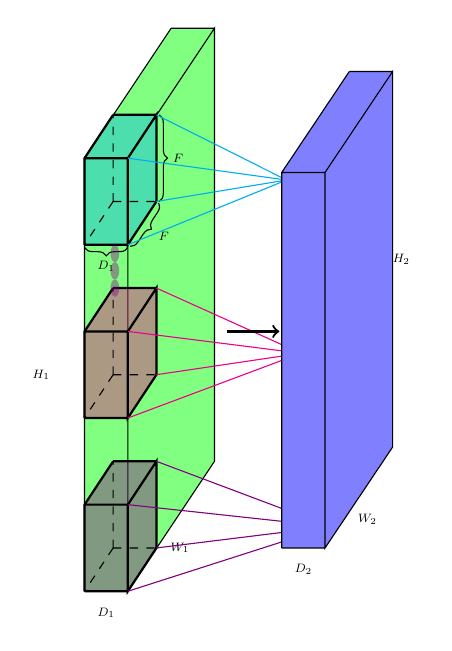
\begin{tikzpicture}[scale=.55, transform shape]
\def\h{10}
\def\w{2}
\def\d{3}
\coordinate (A) at (0,0);
\coordinate (B) at (0,\h);
\coordinate (C) at (\w,\h+\d);
\coordinate (D) at (\w,\d);

\coordinate (A1) at (0+1,0);
\coordinate (B1) at (0+1,\h);
\coordinate (C1) at (\w+1,\h+\d);
\coordinate (D1) at (\w+1,\d);


\fill [draw=none, fill=green!50] (A) -- (B) -- (C) -- (C1) -- (D1) -- (A1) -- cycle; 

\draw (A) -- (B) -- (C) (A) -- (A1) (B) -- (B1) (C) -- (C1) (A1) -- (B1) -- (C1) -- (D1) -- cycle;

\onslide<3->{
\draw [color=white,decorate,decoration={brace,amplitude=10pt,raise=1pt},xshift=0pt,yshift=0pt] (A) -- (B) node [black,midway,xshift=-1cm] {\footnotesize $H_1$};
}
\onslide<4->{
\draw [color=white,decorate,decoration={brace,amplitude=3pt,raise=1pt},xshift=-4pt,yshift=0pt] (A1) -- (A) node [black,midway,yshift=-0.5cm] {\footnotesize $D_1$};
}
\onslide<2->{
\draw [color=white, decorate,decoration={brace,amplitude=10pt,mirror,raise=1pt},xshift=0pt,yshift=0pt] (A1) -- (D1) node [black,midway,xshift=0.2cm,yshift=-0.5cm] {\footnotesize $W_1$};
}

\def\ha{2}
\def\wa{0.66}
\def\sa{1}
\def\wb{0.33}%shift
\def\sb{0.5}%shift
\def\hc{0.66}%next layer box
\def\wc{0.22}%next layer box size
\def\sc{0.33}
\def\xm{4} %distance of next box
\def\xmv{0.22}
\def\ymv{1}
\def\wid{1}
%\def\mycolor{red}

\edef\y{8}
\edef\x{0}


		%feature map 1, points
		\coordinate (A4) at (0+\x*\wb+\xm+\xmv,0+\y+\x*\sb+\ymv);
		\coordinate (B4) at (0+\x*\wb+\xm+\xmv,\hc+\y+\x*\sb+\ymv);
		\coordinate (C4) at (\wc+\x*\wb+\xm+\xmv,\hc+\sc+\y+\x*\sb+\ymv);
		\coordinate (D4) at (\wc+\x*\wb+\xm+\xmv,\sc+\y+\x*\sb+\ymv);
		%\edef\xta{\wc*0.5+\x*\wb+\xm+\xmv}
		%\edef\yta{\y+\x*\sb+\ymv+\hc*0.5+\sc*0.5}		


		

%\foreach \mycolor [count=\xi from 1] [count=\yi from 2] in {cyan,magenta,orange,violet}{				
		\onslide<6->{
		\edef\mycolor{cyan}
		\edef\myval{0.3333}		
		\edef\y{8}
		%\edef\x{\xi}
		%layer1 feature map coordinates
		\coordinate (A6) at (0+\xm+\xmv+\myval,0+\ymv);
		\coordinate (B6) at (0+\xm+\xmv+\myval,\h-\sc);
		\coordinate (C6) at (\w+\xm-\xmv+\myval,\h+\d-\ymv);
		\coordinate (D6) at (\w+\xm-\xmv+\myval,\d+\sc);		
		
		\coordinate (A2) at (0+\x*\wb,0+\y+\x*\sb);
		\coordinate (B2) at (0+\x*\wb,\ha+\y+\x*\sb);
		\coordinate (C2) at (\wa+\x*\wb,\ha+\sa+\y+\x*\sb);
		\coordinate (D2) at (\wa+\x*\wb,\sa+\y+\x*\sb);
		
		\coordinate (A3) at (0+1+\x*\wb,0+\y+\x*\sb);
		\coordinate (B3) at (0+1+\x*\wb,\ha+\y+\x*\sb);
		\coordinate (C3) at (\wa+1+\x*\wb,\ha+\sa+\y+\x*\sb);
		\coordinate (D3) at (\wa+1+\x*\wb,\sa+\y+\x*\sb);		
		
		
		\coordinate (ABCD4) at (\wc*0.5+\x*\wb+\xm+\xmv+\myval,\y+\x*\sb+\ymv+\hc*0.5+\sc*0.5);

		\fill [draw=none, fill=\mycolor, fill opacity=0.4] (A2) -- (B2) -- (C2) -- (C3) -- (D3) -- (A3) -- cycle; 
			
		\draw[thick] (A2) -- (B2) -- (C2) (A2) -- (A3) (B2) -- (B3) (C2) -- (C3) (A3) -- (B3) -- (C3) -- (D3) -- cycle;
		\draw[dashed] (D2) -- (A2) (D2) -- (C2) (D2) -- (D3);
	\onslide<8->{
\draw [decorate,decoration={brace,amplitude=3pt,raise=1pt},xshift=0pt,yshift=0pt] (C3) -- (D3) node [black,midway,xshift=0.5cm] {\footnotesize $F$};

\draw [decorate,decoration={brace,amplitude=3pt,raise=1pt},xshift=-4pt,yshift=0pt] (A3) -- (A2) node [black,midway,yshift=-0.5cm] {\footnotesize $D_1$};

\draw [decorate,decoration={brace,amplitude=3pt,mirror,raise=1pt},xshift=0pt,yshift=0pt] (A3) -- (D3) node [black,midway,xshift=0.5cm,yshift=-0.3cm] {\footnotesize $F$};		
	}
		
		\onslide<7->{
		\draw[\mycolor] (A3) -- (ABCD4) (B3) -- (ABCD4) (C3) -- (ABCD4) (D3) -- (ABCD4);
		
		\fill[\mycolor] (ABCD4) ellipse (0.1 and 0.2);
		}
		\onslide<7->{
		\fill [draw=none, fill=\mycolor] (A6) -- (B6) -- (C6) --  (D6) -- cycle;			
		}
		
		}	
		
		\onslide<7->{
		\edef\mycolor{magenta}
		\edef\myval{2*0.3333}		
		\edef\y{4}
		%\edef\x{\xi}
		%layer1 feature map coordinates
		\coordinate (A26) at (0+\xm+\xmv+\myval,0+\ymv);
		\coordinate (B26) at (0+\xm+\xmv+\myval,\h-\sc);
		\coordinate (C26) at (\w+\xm-\xmv+\myval,\h+\d-\ymv);
		\coordinate (D26) at (\w+\xm-\xmv+\myval,\d+\sc);		
		
		\coordinate (A22) at (0+\x*\wb,0+\y+\x*\sb);
		\coordinate (B22) at (0+\x*\wb,\ha+\y+\x*\sb);
		\coordinate (C22) at (\wa+\x*\wb,\ha+\sa+\y+\x*\sb);
		\coordinate (D22) at (\wa+\x*\wb,\sa+\y+\x*\sb);
		
		\coordinate (A23) at (0+1+\x*\wb,0+\y+\x*\sb);
		\coordinate (B23) at (0+1+\x*\wb,\ha+\y+\x*\sb);
		\coordinate (C23) at (\wa+1+\x*\wb,\ha+\sa+\y+\x*\sb);
		\coordinate (D23) at (\wa+1+\x*\wb,\sa+\y+\x*\sb);		
		
		
		\coordinate (ABCD24) at (\wc*0.5+\x*\wb+\xm+\xmv+\myval,\y+\x*\sb+\ymv+\hc*0.5+\sc*0.5);

		\fill [draw=none, fill=\mycolor, fill opacity=0.4] (A22) -- (B22) -- (C22) -- (C23) -- (D23) -- (A23) -- cycle; 
			
		\draw[thick] (A22) -- (B22) -- (C22) (A22) -- (A23) (B22) -- (B23) (C22) -- (C23) (A23) -- (B23) -- (C23) -- (D23) -- cycle;
		\draw[dashed] (D22) -- (A22) (D22) -- (C22) (D22) -- (D23);
		
		\onslide<7->{
		\draw[\mycolor] (A23) -- (ABCD24) (B23) -- (ABCD24) (C23) -- (ABCD24) (D23) -- (ABCD24);
		
		\fill[\mycolor] (ABCD24) ellipse (0.1 and 0.2);
		}
		\onslide<7->{
		\fill [draw=none, fill=\mycolor] (A26) -- (B26) -- (C26) --  (D26) -- cycle;			
		}	
		
		}
		
		\onslide<7->{
		\edef\mycolor{violet}		
		\fill[\mycolor,fill opacity=0.4] (0.7+\x*\wb,0+\y+\x*\sb-0.2) ellipse (0.1 and 0.2);
		\fill[\mycolor,fill opacity=0.4] (0.7+\x*\wb,0+\y+\x*\sb-0.6) ellipse (0.1 and 0.2);
		\fill[\mycolor,fill opacity=0.4] (0.7+\x*\wb,0+\y+\x*\sb-1) ellipse (0.1 and 0.2);
		}
		\onslide<7->{
		\edef\myval{4*0.3333}		
		\edef\y{0}
		%\edef\x{\xi}
		%layer1 feature map coordinates
		\coordinate (A16) at (0+\xm+\xmv+\myval,0+\ymv);
		\coordinate (B16) at (0+\xm+\xmv+\myval,\h-\sc);
		\coordinate (C16) at (\w+\xm-\xmv+\myval,\h+\d-\ymv);
		\coordinate (D16) at (\w+\xm-\xmv+\myval,\d+\sc);		
		
		\coordinate (A12) at (0+\x*\wb,0+\y+\x*\sb);
		\coordinate (B12) at (0+\x*\wb,\ha+\y+\x*\sb);
		\coordinate (C12) at (\wa+\x*\wb,\ha+\sa+\y+\x*\sb);
		\coordinate (D12) at (\wa+\x*\wb,\sa+\y+\x*\sb);
		
		\coordinate (A13) at (0+1+\x*\wb,0+\y+\x*\sb);
		\coordinate (B13) at (0+1+\x*\wb,\ha+\y+\x*\sb);
		\coordinate (C13) at (\wa+1+\x*\wb,\ha+\sa+\y+\x*\sb);
		\coordinate (D13) at (\wa+1+\x*\wb,\sa+\y+\x*\sb);		
		
		
		\coordinate (ABCD14) at (\wc*0.5+\x*\wb+\xm+\xmv+\myval,\y+\x*\sb+\ymv+\hc*0.5+\sc*0.5);

		\fill [draw=none, fill=\mycolor, fill opacity=0.4] (A12) -- (B12) -- (C12) -- (C13) -- (D13) -- (A13) -- cycle; 
			
		\draw[thick] (A12) -- (B12) -- (C12) (A12) -- (A13) (B12) -- (B13) (C12) -- (C13) (A13) -- (B13) -- (C13) -- (D13) -- cycle;
		\draw[dashed] (D12) -- (A12) (D12) -- (C12) (D12) -- (D13);
		
		%\draw [decorate,decoration={brace,amplitude=12pt,raise=1pt},xshift=0pt,yshift=0pt] (A3) -- (B13) node [black,midway,xshift=1.4cm] {\footnotesize $K$ filters};		
		
		}
		\onslide<7->{
		\draw[\mycolor] (A13) -- (ABCD14) (B13) -- (ABCD14) (C13) -- (ABCD14) (D13) -- (ABCD14);
		
		\fill[\mycolor] (ABCD14) ellipse (0.1 and 0.2);
		}
		\onslide<7->{
		\fill [draw=none, fill=\mycolor] (A16) -- (B16) -- (C16) --  (D16) -- cycle;	
		}
		
		
		\onslide<9->{
			\fill [draw=none, fill=blue!50] (A6) -- (B6) -- (C6) -- (C16) -- (D16) -- (A16) -- cycle;			
			\draw (A6) -- (B6) -- (C6) (A6) -- (A16) (B6) -- (B16) (C6) -- (C16) (A16) -- (B16) -- (C16) -- (D16) -- cycle;
			
		\draw[thick,->] (3.3,6) -- (4.5,6);
\draw [color=white, decorate,decoration={brace,amplitude=10pt,raise=1pt},xshift=0pt,yshift=0pt] (C16) -- (D16) node [black,midway,xshift=0.2cm] {\footnotesize $H_2$};

\draw [color=white, decorate,decoration={brace,amplitude=3pt,raise=1pt},xshift=-4pt,yshift=0pt] (A16) -- (A6) node [black,midway,yshift=-0.5cm] {\footnotesize $D_2$};

\draw [color=white, decorate,decoration={brace,amplitude=10pt,mirror,raise=1pt},xshift=0pt,yshift=0pt] (A16) -- (D16) node [black,midway,xshift=0.2cm,yshift=-0.5cm] {\footnotesize $W_2$};
		}
%}


\end{tikzpicture}
\end{center}
		\end{overlayarea}
		
		\column{0.5\textwidth}
		\begin{overlayarea}{\textwidth}{\textheight}
			\justifying
			\begin{itemize}
			\justifying
				\item We first define the following quantities
				      \item<2-> Width ($W_1$), \onslide<3->{ Height ($H_1$) \onslide<4->{ and Depth ($D_1$) of the original input}}
				      \item<5-> The Stride $S$ (We will come back to this later)
				      \item<7-> The number of filters $K$ 
				      \item<8-> The spatial extent ($F$) of each filter (the depth of each filter is same as the depth of each input)
				      \item<9-> The output is $W_2 \times H_2 \times D_2$ (we will soon see a formula for computing $W_2$, $H_2$ and $D_2$)
			\end{itemize}
			
			
			
		\end{overlayarea}
	\end{columns}
\end{frame}

%%%%%%%%%%%%%%%%%%%%%%%%%%%%%%%%%%%%%%%%%%%%%%%%%%%%%%%%%%%%%%%%%%%%%%%%%%%%%%

\begin{frame}
	\begin{columns}
		\column{0.5\textwidth}
		\begin{overlayarea}{\textwidth}{\textheight}
			\begin{minipage}[t]{0.5\textwidth}
				
				%\resizebox{1\textwidth}{1\textwidth}
			\end{minipage}
			\begin{minipage}[t]{0.5\textwidth}
				\vspace{30mm}
				%\tiny{
				%\begin{align*}
				%\begin{split}
				%    \onslide<11->{
				%        W_2=\frac{W_1-F}{S}+1 \\
				%        H_2=\frac{H_1-F}{S}+1
				%        }
				%\end{split}
				%\end{align*}
				%}
			\end{minipage}
			              
		\end{overlayarea}
		        
		\column{0.5\textwidth}<1->
		\begin{overlayarea}{\textwidth}{\textheight}
			\footnotesize{
				\begin{itemize}
					\justifying
					\item<1-> Let us compute the dimension ($W_2, H_2$) of the output
					\item<8-> Notice that we can't place the kernel at the corners as it will cross the input boundary
					\item<10-> This is true for all the shaded points (the kernel crosses the input boundary)
					\item<11-> This results in an output which is of smaller dimensions than the input
				\end{itemize}}
		\end{overlayarea}
	\end{columns}
\end{frame}

%%%%%%%%%%%%%%%%%%%%%%%%%%%%%%%%%%%%%%%%%%%%%%%%%%%%%%%%%%%%%%%%%%%%%%%%%%%%%%
\begin{frame}
    \begin{columns}
        \column{0.5\textwidth}
        \begin{overlayarea}{\textwidth}{\textheight}
          \begin{minipage}[t]{0.5\textwidth}

%\resizebox{1\textwidth}{1\textwidth}{%
    		\begin{tikzpicture}[remember picture,overlay,shift={(current page.center)}]
  \tikzset{
    mstyle/.style={column sep=-\pgflinewidth,row sep=-\pgflinewidth,font=\footnotesize,},
    window/.style={draw,very thick,blue},
  }
  
  \only<1>{
			\matrix(convmat1) at (-6,2.5) [matrix of nodes,ampersand replacement=\&,column sep=-\pgflinewidth,row sep=-\pgflinewidth,nodes in empty cells,
			nodes={draw,rectangle, font=\footnotesize,anchor=south}]{
				|[fill=black!50]| \& |[fill=black!50]| \& |[fill=black!50]| \& |[fill=black!50]| \& |[fill=black!50]| \& |[fill=black!50]| \& |[fill=black!50]|\\ 
				|[fill=black!50]|\&  \&  \&  \&  \&  \&|[fill=black!50]| \\ 
				|[fill=black!50]|\&  \&  \&  \&  \&  \& |[fill=black!50]|\\ 
				|[fill=black!50]| \&  \&  \&  \&  \&  \& |[fill=black!50]|\\ 
				|[fill=black!50]|\&  \&  \&  \&  \&  \& |[fill=black!50]|\\ 
				|[fill=black!50]| \&  \&  \&  \&  \&  \& |[fill=black!50]|\\ 
				|[fill=black!50]|\& |[fill=black!50]| \& |[fill=black!50]| \&  |[fill=black!50]|\&|[fill=black!50]|  \&  |[fill=black!50]|\& |[fill=black!50]|\\ 
			};
 

			% \matrix (mat1) at (-5.23,1.73)  [matrix of nodes,ampersand replacement=\&,
			%   nodes={draw=blue,rectangle},nodes in empty cells]
			%   {
			%      \&  \&  \\
			%      \&  \&  \\
			%      \&  \&  \\
			%   };
			%            \node (text) [below of = mat1, node distance = 3 em, anchor=east]{\footnotesize \textsf{pixel of interest}};
			%               \draw[<-, in=0, out=-90] (-5.23,1.73) to (text.north);  
        
			\matrix(convmat2)[right of=convmat1,node distance=6em,matrix of nodes,ampersand replacement=\&,column sep=-\pgflinewidth,row sep=-\pgflinewidth,nodes in empty cells,
			nodes={draw,rectangle, font=\footnotesize,anchor=south}]{
				\&  \&  \& \& \\
				\&  \&  \& \& \\
				\&  \&  \& \& \\
				\&  \&  \&  \& \\
				\&  \&  \&  \& \\
			};
			
			
			\foreach \i  in {1,...,5}{
				\foreach \j  in {1,...,5}{

					\draw[fill=black] (convmat2-\i-\j)circle(1.5pt);

				}
			}

			\node(text)[left of = convmat2,node distance=2em, anchor=east]{\footnotesize \textsf{=}}; 
		}
              \onslide<2-4>{
              \matrix(convmat1) at (-6,2.5)[matrix of nodes,ampersand replacement=\&,column sep=-\pgflinewidth,row sep=-\pgflinewidth,nodes in empty cells,
                nodes={draw,rectangle, font=\footnotesize,anchor=south}]{
                     \&  \&  \&  \&  \&  \& \\ 
	   \&  \&  \&  \&  \&  \& \\ 
	   \&  \&  \&  \&  \&  \& \\ 
	   \&  \&  \&  \&  \&  \& \\ 
	   \&  \&  \&  \&  \&  \& \\ 
	  \&  \&  \&  \&  \&  \& \\ 
	   \&  \&  \&  \&  \&  \& \\ 
	              };
	
	 
	  % \foreach \i/\j [count=\xi from 0] in {1/3,2/4,3/5,4/6,5/7,6/8,7/9,8/10,9/11,10/12,11/13,12/14,13/15,14/16,15/17,16/18,17/19,18/20,19/21,20/22,21/23,22/24,23/25,24/26,25/27,26/28}{
	  %   \foreach \k/\m [count=\yi from \xi*26+1] in {1/3,2/4,3/5,4/6,5/7,6/8,7/9,8/10,9/11,10/12,11/13,12/14,13/15,14/16,15/17,16/18,17/19,18/20,19/21,20/22,21/23,22/24,23/25,24/26,25/27,26/28}{
	  %    \onslide<\yi>{
	  %    \draw[window](convmat1-\i-\k.north west)rectangle(convmat1-\j-\m.south east);
	     
	  %    }
	  %   }
	  % }
	\foreach \i/\j [count=\xi from 2] in {1/5,2/6,3/7}{
	\onslide<\xi>{
	  \draw[window](convmat1-1-\i.north west)rectangle(convmat1-5-\j.south east);
	}
	  
	}
	              
	              
	              \matrix(convmat2)[right of=convmat1,node distance=6em,matrix of nodes,ampersand replacement=\&,column sep=-\pgflinewidth,row sep=-\pgflinewidth,nodes in empty cells,
	                nodes={draw,rectangle, font=\footnotesize,anchor=south}]{
	       \&  \&  \\
	       \&  \&  \\
	       \&  \&  \\
	    };
	
	 
	  % \foreach \i [count=\xi from 0] in {1,...,5}{
	  %             \foreach \j [count=\yi from \xi*5+1] in {1,...,5}{
	    % \onslide<\yi->{
	  %             \draw[fill=black] (convmat2-\i-\j)circle(1.5pt);
	    % }
	  %             }
	  %             }
	  \foreach \i/\j [count=\xi from 2] in {1/1,2/2,3/3}{
	  \onslide<\xi->{
	    \draw[fill=black] (convmat2-1-\j)circle(1.5pt);
	  }
	
	  }
	\node(text)[left of = convmat2,node distance=2em, anchor=east]{\footnotesize \textsf{=}}; 
	}
	
	\only<5>{
	              \matrix(convmat1) at (-6,2.5) [matrix of nodes,ampersand replacement=\&,column sep=-\pgflinewidth,row sep=-\pgflinewidth,nodes in empty cells,
	                nodes={draw,rectangle, font=\footnotesize,anchor=south}]{
	                     \&  \&  \&  \&  \&  \& \\ 
	   \&  \&  \&  \&  \&  \& \\ 
	   \&  \&  \&  \&  \&  \& \\ 
	   \&  \&  \&  \&  \&  \& \\ 
	   \&  \&  \&  \&  \&  \& \\ 
	  \&  \&  \&  \&  \&  \& \\ 
	   \&  \&  \&  \&  \&  \& \\ 
	              };
	 
	  \draw[window](convmat1-3-3.north west)rectangle(convmat1-7-7.south east);
	              
	              
	              \matrix(convmat2)[right of=convmat1,node distance=6em,matrix of nodes,ampersand replacement=\&,column sep=-\pgflinewidth,row sep=-\pgflinewidth,nodes in empty cells,
	                nodes={draw,rectangle, font=\footnotesize,anchor=south}]{
	       \&  \&  \\
	       \&  \&  \\
	       \&  \&  \\
	    };
	
	
	 \foreach \i  in {1,...,3}{
	              \foreach \j  in {1,...,3}{
	    
	              \draw[fill=black] (convmat2-\i-\j)circle(1.5pt);
	    
	              }
	              }
	  
	\node(text)[left of = convmat2,node distance=2em, anchor=east]{\footnotesize \textsf{=}}; 
	}
	\only<6>{
	              \matrix(convmat1) at (-6,2.5) [matrix of nodes,ampersand replacement=\&,column sep=-\pgflinewidth,row sep=-\pgflinewidth,nodes in empty cells,
	                nodes={draw,rectangle, font=\footnotesize,anchor=south}]{
	                     \&  \&  \&  \&  \&  \& \\ 
	   \&  \&  \&  \&  \&  \& \\ 
	   \&  \&  \&  \&  \&  \& \\ 
	   \&  \&  \&  \&  \&  \& \\ 
	   \&  \&  \&  \&  \&  \& \\ 
	  \&  \&  \&  \&  \&  \& \\ 
	   \&  \&  \&  \&  \&  \& \\ 
	              };
 
  %\draw[window](convmat1-6-6.north west)rectangle($(convmat1-7-7.south east)+(-1,-1)$);
  \matrix (mat1) at (-5.48,1.98)  [matrix of nodes,ampersand replacement=\&,
    nodes={draw=blue,rectangle},nodes in empty cells]
    {
       \&  \&  \& \& \\
       \&  \&  \& \& \\
       \&  \&  \& \& \\
       \&  \&  \&  \& \\
       \&  \&  \&  \& \\
    };
    

    \node (text) [below of = mat1, node distance = 3 em, anchor=east]{\footnotesize \textsf{pixel of interest}};
                \draw[<-, in=0, out=-90] (-5.485,1.975) to (text.north);
              
              \matrix(convmat2)[right of=convmat1,node distance=6em,matrix of nodes,ampersand replacement=\&,column sep=-\pgflinewidth,row sep=-\pgflinewidth,nodes in empty cells,
                nodes={draw,rectangle, font=\footnotesize,anchor=south}]{
       \&  \&  \\
       \&  \&  \\
       \&  \&  \\
    };


	 \foreach \i  in {1,...,3}{
	              \foreach \j  in {1,...,3}{
	    
	              \draw[fill=black] (convmat2-\i-\j)circle(1.5pt);
	    
	              }
	              }
	  
	\node(text)[left of = convmat2,node distance=2em, anchor=east]{\footnotesize \textsf{=}}; 
	}
	
	
	
	\only<7>{
	              \matrix(convmat1) at (-6,2.5) [matrix of nodes,ampersand replacement=\&,column sep=-\pgflinewidth,row sep=-\pgflinewidth,nodes in empty cells,
	                nodes={draw,rectangle, font=\footnotesize,anchor=south}]{
	                     \&  \&  \&  \&  \&  \& \\ 
	   \&  \&  \&  \&  \&  \& \\ 
	   \&  \&  \&  \&  \&  \& \\ 
	   \&  \&  \&  \&  \&  \& \\ 
	   \&  \&  \&  \&  \&  \& \\ 
	  \&  \&  \&  \&  \&  \& \\ 
	   \&  \&  \&  \&  \&  \& \\ 
	              };
	 
	  %\draw[window](convmat1-6-6.north west)rectangle($(convmat1-7-7.south east)+(-1,-1)$);
	  \matrix (mat1) at (-5.22,1.72)  [matrix of nodes,ampersand replacement=\&,
	    nodes={draw=blue,rectangle},nodes in empty cells]
	    {
	       \&  \&  \& \& \\
	       \&  \&  \& \& \\
	       \&  \&  \& \& \\
	       \&  \&  \&  \& \\
	       \&  \&  \&  \& \\
	    };
	    
	
	    \node (text) [below of = mat1, node distance = 3 em, anchor=east]{\footnotesize \textsf{pixel of interest}};
	                \draw[<-, in=0, out=-90] (-5.22,1.72) to (text.north);
	              
	              \matrix(convmat2)[right of=convmat1,node distance=6em,matrix of nodes,ampersand replacement=\&,column sep=-\pgflinewidth,row sep=-\pgflinewidth,nodes in empty cells,
	                nodes={draw,rectangle, font=\footnotesize,anchor=south}]{
	       \&  \&  \\
	       \&  \&  \\
	       \&  \&  \\
	    };
	
	
	 \foreach \i  in {1,...,3}{
	              \foreach \j  in {1,...,3}{
	    
	              \draw[fill=black] (convmat2-\i-\j)circle(1.5pt);
	    
	              }
	              }
	  
	\node(text)[left of = convmat2,node distance=2em, anchor=east]{\footnotesize \textsf{=}}; 
	}
	
	
	\onslide<8->{
	              \matrix(convmat1) at (-6,2.5) [matrix of nodes,ampersand replacement=\&,column sep=-\pgflinewidth,row sep=-\pgflinewidth,nodes in empty cells,
	                nodes={draw,rectangle, font=\footnotesize,anchor=south}]{
	                    |[fill=black!50]| \& |[fill=black!50]| \& |[fill=black!50]| \& |[fill=black!50]| \& |[fill=black!50]| \& |[fill=black!50]| \& |[fill=black!50]|\\ 
	   |[fill=black!50]|\& |[fill=black!30]| \& |[fill=black!30]| \& |[fill=black!30]| \& |[fill=black!30]| \& |[fill=black!30]|  \&|[fill=black!50]| \\ 
	   |[fill=black!50]|\& |[fill=black!30]| \&  \&  \&  \& |[fill=black!30]| \& |[fill=black!50]|\\ 
	  |[fill=black!50]| \& |[fill=black!30]| \&  \&  \&  \& |[fill=black!30]| \& |[fill=black!50]|\\ 
	   |[fill=black!50]|\& |[fill=black!30]| \&  \&  \&  \& |[fill=black!30]| \& |[fill=black!50]|\\ 
	 |[fill=black!50]| \& |[fill=black!30]| \&  |[fill=black!30]|\& |[fill=black!30]| \& |[fill=black!30]| \& |[fill=black!30]| \& |[fill=black!50]|\\ 
	   |[fill=black!50]|\& |[fill=black!50]| \& |[fill=black!50]| \&  |[fill=black!50]|\&|[fill=black!50]|  \&  |[fill=black!50]|\& |[fill=black!50]|\\ 
	              };
	 
	  %\draw[window](convmat1-6-6.north west)rectangle($(convmat1-7-7.south east)+(-1,-1)$);
	  % \matrix (mat1) at (-5.22,1.72)  [matrix of nodes,ampersand replacement=\&,
	  %   nodes={draw=blue,rectangle},nodes in empty cells]
	  %   {
	  %      \&  \&  \& \& \\
	  %      \&  \&  \& \& \\
	  %      \&  \&  \& \& \\
	  %      \&  \&  \&  \& \\
	  %      \&  \&  \&  \& \\
	  %   };
	    
	
	  %   \node (text) [below of = mat1, node distance = 3 em, anchor=east]{\footnotesize \textsf{pixel of interest}};
	  %               \draw[<-, in=0, out=-90] (-5.22,1.72) to (text.north);
	              
	              \matrix(convmat2)[right of=convmat1,node distance=6em,matrix of nodes,ampersand replacement=\&,column sep=-\pgflinewidth,row sep=-\pgflinewidth,nodes in empty cells,
	                nodes={draw,rectangle, font=\footnotesize,anchor=south}]{
	       \&  \&  \\
	       \&  \&  \\
	       \&  \&  \\
	    };
	
	
	 \foreach \i  in {1,...,3}{
	              \foreach \j  in {1,...,3}{
	    
	              \draw[fill=black] (convmat2-\i-\j)circle(1.5pt);
	    
	              }
	              }
	  
	\node(text)[left of = convmat2,node distance=2em, anchor=east]{\footnotesize \textsf{=}}; 
	}

\end{tikzpicture}
%}
  \end{minipage}
\begin{minipage}[t]{0.5\textwidth}
\vspace{30mm}
%\tiny{
\begin{align*}
    %\begin{split}
    \onslide<8->{
        \textit{In general, }
        W_2=W_1-F+1 \\
        H_2=H_1-F+1 \\
        \textit{We will refine this formula further}
        }
    %\end{split}
\end{align*}
%}
\end{minipage}
              
        \end{overlayarea}
        
        \column{0.5\textwidth}<1->
        \begin{overlayarea}{\textwidth}{\textheight}
            \footnotesize{
            \begin{itemize}
                \justifying
                \item<1-> Let us compute the dimension ($W_2, H_2$) of the output
                \item<1-> Notice that we can't place the kernel at the corners as it will cross the input boundary
                \item<1-> This is true for all the shaded points (the kernel crosses the input boundary)
                \item<1-> This results in an output which is of smaller dimensions than the input
                \item<1-> As the size of the kernel increases, this becomes true for even more pixels 
                \item<2-> For example, let's consider a 5 $\times$ 5 kernel
                \item<3-> We have an even smaller output now 
            \end{itemize}}
        \end{overlayarea}
    \end{columns}
\end{frame}

%%%%%%%%%%%%%%%%%%%%%%%%%%%%%%%%%%%%%%%%%%%%%%%%%%%%%%%%%%%%%%%%%%%%%%%%%%%%%%%%%%%%%%%%%%

\begin{frame}
	\begin{columns}
		\column{0.5\textwidth}<1->
		\begin{overlayarea}{\textwidth}{\textheight}
			\begin{minipage}[t]{0.15\textwidth}
				\vspace{2mm}
				%\resizebox{7\textwidth}{5\textwidth}{%
				\begin{tikzpicture}
	\tikzset{
		mstyle/.style={column sep=-\pgflinewidth,row sep=-\pgflinewidth,font=\footnotesize,},
		window/.style={draw,very thick,blue},
	}
	\onslide<4->{
		\matrix(convmat1)[matrix of nodes,ampersand replacement=\&,column sep=-\pgflinewidth,row sep=-\pgflinewidth,nodes in empty cells,
		nodes={draw,rectangle, font=\tiny,minimum height=4mm,minimum width=4mm,anchor=south}]{
			0\&  0\&  0\&  0\& 0\& 0\& 0\& 0\&0\\ 
			0\&  \&  \&  \&  \&  \& \& \&0\\ 
			0\&  \&  \&  \&  \&  \& \& \&0\\ 
			0\&  \&  \&  \&  \&  \& \& \&0\\ 
			0\&  \&  \&  \&  \&  \& \& \&0\\ 
			0\&  \&  \&  \&  \&  \& \& \&0\\ 
			0\&  \&  \&  \&  \&  \& \& \&0\\ 
			0\&  \&  \&  \&  \&  \& \& \&0\\ 
			0\&  0\&  0\&  0\&  0\& 0 \&  0\& 0\&0\\
		};
		
		

		% \foreach \i/\j [count=\xi from 0] in {1/3,2/4,3/5,4/6,5/7,6/8,7/9,8/10,9/11,10/12,11/13,12/14,13/15,14/16,15/17,16/18,17/19,18/20,19/21,20/22,21/23,22/24,23/25,24/26,25/27,26/28,27/29}{
		%   \foreach \k/\m [count=\yi from \xi*27+1] in {1/3,2/4,3/5,4/6,5/7,6/8,7/9,8/10,9/11,10/12,11/13,12/14,13/15,14/16,15/17,16/18,17/19,18/20,19/21,20/22,21/23,22/24,23/25,24/26,25/27,26/28,27/29}{
		%    \onslide<\yi>{
		%    \draw[window](convmat1-\i-\k.north west)rectangle(convmat1-\j-\m.south east);

		%    }
		%   }
		% }
		
		\foreach \i/\j [count=\xi from 4] in {1/3,2/4,3/5,4/6,5/7}{
			\onslide<\xi>{
				\draw[window](convmat1-1-\i.north west)rectangle(convmat1-3-\j.south east);
			}

		}              
    
		\matrix(convmat2)[right of=convmat1,node distance=10em,matrix of nodes,ampersand replacement=\&,column sep=-\pgflinewidth,row sep=-\pgflinewidth,nodes in empty cells,
		nodes={draw,rectangle, font=\footnotesize,anchor=south,minimum height=4mm,minimum width=4mm}]{
			\&  \&  \&  \&  \&  \& \\ 
			\&  \&  \&  \&  \&  \& \\ 
			\&  \&  \&  \&  \&  \& \\ 
			\&  \&  \&  \&  \&  \& \\ 
			\&  \&  \&  \&  \&  \& \\ 
			\&  \&  \&  \&  \&  \& \\ 
			\&  \&  \&  \&  \&  \& \\ 
		};
		
		

		% \foreach \i [count=\xi from 0] in {1,...,28}{
		%             \foreach \j [count=\yi from \xi*28+1] in {1,...,28}{
		% \onslide<\yi->{
		%             \draw[fill=black] (convmat2-\i-\j)circle(1.5pt);
		% }
		%             }
		%             }
		\foreach \i/\j [count=\xi from 4] in {1/1,2/2,3/3,4/4,5/5}{
			\onslide<\xi->{
				\draw[fill=black] (convmat2-1-\j)circle(1.5pt);
			}
			
		}
		
		\node(text)[left of = convmat2,node distance=4em, anchor=east]{\footnotesize \textsf{=}};   
	}%end of 2-6
	\only<9->{
		\matrix(convmat1)[matrix of nodes,ampersand replacement=\&,column sep=-\pgflinewidth,row sep=-\pgflinewidth,nodes in empty cells,
		nodes={draw,rectangle, font=\tiny,minimum height=4mm,minimum width=4mm,anchor=south}]{
			0\&  0\&  0\&  0\& 0\& 0\& 0\& 0\&0\\ 
			0\&  \&  \&  \&  \&  \& \& \&0\\ 
			0\&  \&  \&  \&  \&  \& \& \&0\\ 
			0\&  \&  \&  \&  \&  \& \& \&0\\ 
			0\&  \&  \&  \&  \&  \& \& \&0\\ 
			0\&  \&  \&  \&  \&  \& \& \&0\\ 
			0\&  \&  \&  \&  \&  \& \& \&0\\ 
			0\&  \&  \&  \&  \&  \& \& \&0\\ 
			0\&  0\&  0\&  0\&  0\& 0 \&  0\& 0\&0\\
		};
		
		

		% \foreach \i/\j [count=\xi from 0] in {1/3,2/4,3/5,4/6,5/7,6/8,7/9,8/10,9/11,10/12,11/13,12/14,13/15,14/16,15/17,16/18,17/19,18/20,19/21,20/22,21/23,22/24,23/25,24/26,25/27,26/28,27/29}{
		%   \foreach \k/\m [count=\yi from \xi*27+1] in {1/3,2/4,3/5,4/6,5/7,6/8,7/9,8/10,9/11,10/12,11/13,12/14,13/15,14/16,15/17,16/18,17/19,18/20,19/21,20/22,21/23,22/24,23/25,24/26,25/27,26/28,27/29}{
		%    \onslide<\yi>{
		%    \draw[window](convmat1-\i-\k.north west)rectangle(convmat1-\j-\m.south east);

		%    }
		%   }
		% }
		\draw[window](convmat1-7-7.north west)rectangle(convmat1-9-9.south east);
		
    
    
		\matrix(convmat2)[right of=convmat1,node distance=10em,matrix of nodes,ampersand replacement=\&,column sep=-\pgflinewidth,row sep=-\pgflinewidth,nodes in empty cells,
		nodes={draw,rectangle, font=\footnotesize,anchor=south,minimum height=4mm,minimum width=4mm}]{
			\&  \&  \&  \&  \&  \& \\ 
			\&  \&  \&  \&  \&  \& \\ 
			\&  \&  \&  \&  \&  \& \\ 
			\&  \&  \&  \&  \&  \& \\ 
			\&  \&  \&  \&  \&  \& \\ 
			\&  \&  \&  \&  \&  \& \\ 
			\&  \&  \&  \&  \&  \& \\ 
		};
		
		

		% \foreach \i [count=\xi from 0] in {1,...,28}{
		%             \foreach \j [count=\yi from \xi*28+1] in {1,...,28}{
		%   \onslide<\yi->{
		%             \draw[fill=black] (convmat2-\i-\j)circle(1.5pt);
		%   }
		%             }
		%             }
		\foreach \i  in {1,...,7}{
			\foreach \j  in {1,...,7}{

				\draw[fill=black] (convmat2-\i-\j)circle(1.5pt);

			}
		}
		\node(text)[left of = convmat2,node distance=4em, anchor=east]{\footnotesize \textsf{=}};   
	}%end of 7
	
\end{tikzpicture}
				%}
			\end{minipage}
			
			\begin{minipage}[t]{0.15\textwidth}
				%\tiny{\hspace{1mm}
				\begin{align*}
					\begin{split}                                
					\onslide<9->{                                
					\textit{We now have,}                        \\
					W_2=W_1-F+2P+1                               \\
					H_2=H_1-F+2P+1                               \\
					\textit{We will refine this formula further} 
					}                                            
					\end{split}                                  
				\end{align*}
				%}
			\end{minipage}
			              
		\end{overlayarea}
		        
		\column{0.5\textwidth}<1->
		\begin{overlayarea}{\textwidth}{\textheight}
			\footnotesize{
				\begin{itemize}
					\justifying
					\item<1-> What if we want the output to be of same size as the input?
					\item<2-> We can use something known as padding
					\item<3-> Pad the inputs with appropriate number of 0 inputs so that you can now apply the kernel at the corners
					\item<4-> Let us use pad P = 1 with a 3 $\times$ 3 kernel
					\item<5-> This means we will add one row and one column of 0 inputs at the top, bottom, left and right
					% \item<8-> For example, $P=1$
					% \tiny{
					% \begin{align*}
					% W_2 &= \frac{W_1-F+2P}{S}+1 \\
					%     &= \frac{W_1 -3 + 2}{1} + 1 = W_1 
					% \end{align*}
					% \begin{align*}
					%     H_2 &= \frac{H_1-F+2P}{S}+1 \\
					%         &= \frac{H_1 -3 + 2}{1} + 1 = H_1 
					% \end{align*}
					% }
					% \item <9-> \textbf{Question:} Suppose $F=5$, what should be the value of $P$ be so that $W_2 = W_1$ and $H_2 = H_1$ ? \onslide<10->{\textbf{$P=2$}}
				\end{itemize}}
		\end{overlayarea}
	\end{columns}
\end{frame}

%%%%%%%%%%%%%%%%%%%%%%%%%%%%%%%%%%%%%%%%%%%%%%%%%%%%%%%%%%%%%%%%%%%%%%%%%%%%%%%%%%%%%%%%%%

\begin{frame}
	\begin{columns}
		\column{0.5\textwidth}<1->
		\begin{overlayarea}{\textwidth}{\textheight}
			
			\only<3->{
				\begin{minipage}[t]{0.15\textwidth}
					%\resizebox{7\textwidth}{5\textwidth}{%
					\begin{tikzpicture}
	\tikzset{
		mstyle/.style={column sep=-\pgflinewidth,row sep=-\pgflinewidth,font=\footnotesize,},
		window/.style={draw,very thick,blue},
	}

	\matrix(convmat1)[matrix of nodes,ampersand replacement=\&,column sep=-\pgflinewidth,row sep=-\pgflinewidth,nodes in empty cells,
	nodes={draw,rectangle, font=\tiny,minimum height=4mm,minimum width=4mm,anchor=south}]{
		0\&  0\&  0\&  0\& 0\& 0\& 0\& 0\&0\\ 
		0\&  \&  \&  \&  \&  \& \& \&0\\ 
		0\&  \&  \&  \&  \&  \& \& \&0\\ 
		0\&  \&  \&  \&  \&  \& \& \&0\\ 
		0\&  \&  \&  \&  \&  \& \& \&0\\ 
		0\&  \&  \&  \&  \&  \& \& \&0\\ 
		0\&  \&  \&  \&  \&  \& \& \&0\\ 
		0\&  \&  \&  \&  \&  \& \& \&0\\ 
		0\&  0\&  0\&  0\&  0\& 0 \&  0\& 0\&0\\
	};
	

	\foreach \i/\j [count=\xi from 0] in {1/3,3/5,5/7,7/9}{%,10/12,13/15,16/18,19/21,22/24,25/27}{
		\foreach \k/\m [count=\yi from \xi*4+3] in {1/3,3/5,5/7,7/9}{%,10/12,13/15,16/18,19/21,22/24,25/27}{
			\onslide<\yi>{
				\draw[window](convmat1-\i-\k.north west)rectangle(convmat1-\j-\m.south east);

			}
		}
	}
	%   \foreach \i/\j [count=\xi from 3] in {1/3,4/6,7/9,10/12,13/15}{
	% \onslide<\xi>{
	%   \draw[window](convmat1-1-\i.north west)rectangle(convmat1-3-\j.south east);
	% }

	% }      
	


	\matrix(convmat2)[right of=convmat1,node distance=10em,matrix of nodes,ampersand replacement=\&,column sep=-\pgflinewidth,row sep=-\pgflinewidth,nodes in empty cells,
	nodes={draw,rectangle, font=\footnotesize,anchor=south,minimum height=4mm,minimum width=4mm}]{
		\&  \&  \& \\
		\&  \&  \& \\
		\&  \&  \& \\
		\&  \&  \&  \\
	};
	
	
	% \foreach \i/\j [count=\xi from 3] in {1/1,2/2,3/3,4/4,5/5}{
	%  \onslide<\xi->{
	%    \draw[fill=black] (convmat2-1-\j)circle(1.5pt);
	%  }
	
	%  }
	\foreach \i [count=\xi from 0] in {1,...,4}{
		\foreach \j [count=\yi from \xi*4+3] in {1,...,4}{
			\onslide<\yi->{
				\draw[fill=black] (convmat2-\i-\j)circle(1.5pt);
			}
		}
	}
	
	\node(text)[left of = convmat2,node distance=3em, anchor=east]{\footnotesize \textsf{=}};   
\end{tikzpicture}
					%}
				\end{minipage}
			}
			%%%%%%%%%%%%%%%%%%%%%%%%%%%%%%%%%%%%%%%%%%%%%%%%%%%%%%%%%%%%%%%%%%%%%%%%%%%%%%%%%%%%%%%%%%%%%%%%%%%%%%%%%%%%%%%%%%%%%%%%%%%%%%%%%%%%%%%%%%%%%%%%%%%%%%%%%
			% \only<8->{
			%           \begin{minipage}[t]{0.15\textwidth}
			% \resizebox{7\textwidth}{5\textwidth}{%
			%     \begin{tikzpicture}
			%               \tikzset{
			%                 mstyle/.style={column sep=-\pgflinewidth,row sep=-\pgflinewidth,font=\footnotesize,},
			%                 window/.style={draw,very thick,blue},
			%               }
			              
			%               \matrix(convmat1)[matrix of nodes,ampersand replacement=\&,column sep=-\pgflinewidth,row sep=-\pgflinewidth,nodes in empty cells,
			%                 nodes={draw,rectangle, font=\tiny,minimum height=4mm,minimum width=4mm,anchor=south}]{
			%                    0\&  0\&  0\&  0\&  0\& 0\& 0\&0\\ 
			%  0\&  \&  \&  \&  \&  \&  \&0\\ 
			%  0\&  \&  \&  \&  \&  \&  \&0\\ 
			%  0\&  \&  \&  \&  \&  \&  \&0\\ 
			%  0\&  \&  \&  \&  \&  \&  \&0\\ 
			%  0\&  \&  \&  \&  \&  \&  \&0\\ 
			%  0\&  \&  \&  \&  \&  \&  \&0\\ 
			%  0\&  0\&  0\&  0\&  0\&   0\& 0\&0\\
			%               };
			
			 
			%   % \foreach \i/\j [count=\xi from 0] in {1/3,4/6,7/9,10/12,13/15,16/18,19/21,22/24,25/27}{
			%   %   \foreach \k/\m [count=\yi from \xi*9+1] in {1/3,4/6,7/9,10/12,13/15,16/18,19/21,22/24,25/27}{
			%   %    \onslide<\yi>{
			%   %    \draw[window](convmat1-\i-\k.north west)rectangle(convmat1-\j-\m.south east);
			     
			%   %    }
			%   %   }
			%   % }
			%   \draw[window](convmat1-27-27.north west)rectangle(convmat1-29-29.south east);
			
			              
			              
			%               \matrix(convmat2)[right of=convmat1,node distance=35em,matrix of nodes,ampersand replacement=\&,column sep=-\pgflinewidth,row sep=-\pgflinewidth,nodes in empty cells,
			%                 nodes={draw,rectangle, font=\footnotesize,anchor=south,minimum height=4mm,minimum width=4mm}]{
			%        \&  \&  \\
			%        \&  \&  \\
			%        \&  \&  \\
			%     };
			
			%  \foreach \i  in {1,...,10}{
			%               \foreach \j  in {1,...,10}{
			    
			%               \draw[fill=black] (convmat2-\i-\j)circle(1.5pt);
			    
			%               }
			%               }
			%   % \foreach \i [count=\xi from 0] in {1,...,10}{
			%   %             \foreach \j [count=\yi from \xi*10+1] in {1,...,10}{
			%   %   \onslide<\yi->{
			%   %             \draw[fill=black] (convmat2-\i-\j)circle(1.5pt);
			%   %   }
			%   %             }
			%   %             }
			  
			% \node(text)[left of = convmat2,node distance=12em, anchor=east]{\footnotesize \textsf{=}};   
			%               \end{tikzpicture}
			% }
			%     \end{minipage}
			% }
			
			
			
			\begin{minipage}[t]{0.15\textwidth}
				\vspace{3mm}
				%\tiny{
				\begin{align*}
					\begin{split}                                                              
					\onslide<17->{        \textit{So what should our final formula look like,} \\}
					\onslide<18->{                                                             
					W_2=\frac{W_1-F+2P}{S}+1                                                   \\
					H_2=\frac{H_1-F+2P}{S}+1                                                   
					}                                                                          
					\end{split}                                                                
				\end{align*}
				%}
			\end{minipage}
			              
		\end{overlayarea}
		        
		\column{0.5\textwidth}<1->
		\begin{overlayarea}{\textwidth}{\textheight}
			\begin{itemize}
				\item<1-> What does the stride S do?
				\item<2-> It defines the intervals at which the filter is applied (here $S=2$)
				\item<3-> Here, we are essentially skipping every 2nd pixel which will again result in an output which is of smaller dimensions
				% \item<9-> For $S=3$
				% \begin{align*}
				%     W_2 &=\frac{W_1-F+2P}{S}+1\\
				%         &= \frac{28 -3 + 2}{3} + 1 = 10
				% \end{align*}
				%  \begin{align*}
				%     H_2 &=\frac{H_1-F+2P}{S}+1\\
				%         &= \frac{28 -3 + 2}{3} + 1 = 10
				%\end{align*}
			\end{itemize}
		\end{overlayarea}
	\end{columns}
\end{frame}

%%%%%%%%%%%%%%%%%%%%%%%%%%%%%%%%%%%%%%%%%%%%%%%%%%%%%%%%%%%%%%%%%%%%%%%%%%%%%%%%%%%%%%%%%%

\begin{frame}
	\begin{columns}
		
		\column{0.5\textwidth}
		\begin{overlayarea}{\textwidth}{\textheight}
			\begin{center}
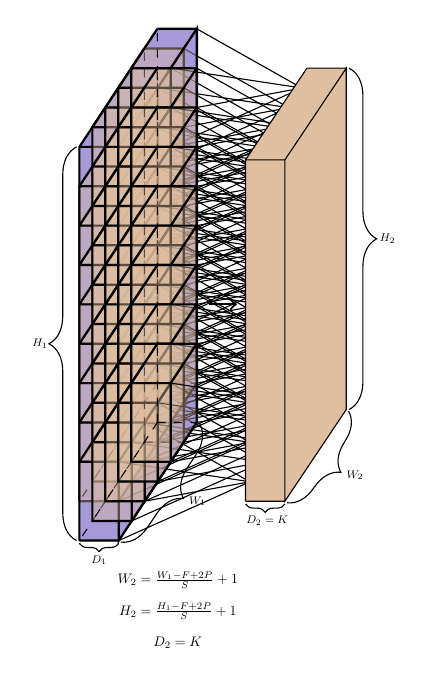
\begin{tikzpicture}[scale=.5, transform shape]
\def\h{10}
\def\w{2}
\def\d{3}
\coordinate (A) at (0,0);
\coordinate (B) at (0,\h);
\coordinate (C) at (\w,\h+\d);
\coordinate (D) at (\w,\d);


\coordinate (A1) at (0+1,0);
\coordinate (B1) at (0+1,\h);
\coordinate (C1) at (\w+1,\h+\d);
\coordinate (D1) at (\w+1,\d);

\fill [draw=none, fill=blue!50] (A) -- (B) -- (C) -- (C1) -- (D1) -- (A1) -- cycle;
\draw (A) -- (B) -- (C) (A) -- (A1) (B) -- (B1) (C) -- (C1) (A1) -- (B1) -- (C1) -- (D1) -- cycle;

\draw [decorate,decoration={brace,amplitude=10pt,raise=1pt},xshift=0pt,yshift=0pt] (A) -- (B) node [black,midway,xshift=-1cm] {\footnotesize $H_1$};

\draw [decorate,decoration={brace,amplitude=3pt,raise=1pt},xshift=-4pt,yshift=0pt] (A1) -- (A) node [black,midway,yshift=-0.5cm] {\footnotesize $D_1$};

\draw [decorate,decoration={brace,amplitude=10pt,mirror,raise=1pt},xshift=0pt,yshift=0pt] (A1) -- (D1) node [black,midway,xshift=1cm,yshift=-0.5cm] {\footnotesize $W_1$};

\def\ha{2}
\def\wa{0.66}
\def\sa{1}
\def\wb{0.33}%shift
\def\sb{0.5}%shift
\def\hc{0.66}%next layer box
\def\wc{0.22}%next layer box size
\def\sc{0.33}
\def\xm{4} %distance of next box
\def\xmv{0.22}
\def\ymv{1}
\def\wid{1}


%layer1 feature map coordinates
\coordinate (A6) at (0+\xm+\xmv,0+\ymv);
\coordinate (B6) at (0+\xm+\xmv,\h-\sc);
\coordinate (C6) at (\w+\xm-\xmv,\h+\d-\ymv);
\coordinate (D6) at (\w+\xm-\xmv,\d+\sc);

\coordinate (A7) at (0+1+\xm+\xmv,0+\ymv);
\coordinate (B7) at (0+1+\xm+\xmv,\h-\sc);
\coordinate (C7) at (\w+1+\xm-\xmv,\h+\d-\ymv);
\coordinate (D7) at (\w+1+\xm-\xmv,\d+\sc);

\fill [draw=none, fill=brown!50] (A6) -- (B6) -- (C6) --  (D6) -- cycle;	


\onslide<1>{
\def\xz{4}
\def\yz{4}
		\coordinate (A2) at (0+\xz*\wb,0+\yz+\xz*\sb);
		\coordinate (B2) at (0+\xz*\wb,\ha+\yz+\xz*\sb);
		\coordinate (C2) at (\wa+\xz*\wb,\ha+\sa+\yz+\xz*\sb);
		\coordinate (D2) at (\wa+\xz*\wb,\sa+\yz+\xz*\sb);
		
		\coordinate (A3) at (0+1+\xz*\wb,0+\yz+\xz*\sb);
		\coordinate (B3) at (0+1+\xz*\wb,\ha+\yz+\xz*\sb);
		\coordinate (C3) at (\wa+1+\xz*\wb,\ha+\sa+\yz+\xz*\sb);
		\coordinate (D3) at (\wa+1+\xz*\wb,\sa+\yz+\xz*\sb);
		
		
		\fill [draw=none, fill=brown!50, fill opacity=0.4] (A2) -- (B2) -- (C2) -- (C3) -- (D3) -- (A3) -- cycle; 
			
		\draw[thick] (A2) -- (B2) -- (C2) (A2) -- (A3) (B2) -- (B3) (C2) -- (C3) (A3) -- (B3) -- (C3) -- (D3) -- cycle;
		\draw[dashed] (D2) -- (A2) (D2) -- (C2) (D2) -- (D3);
		
		\node[] (input1) at (0+0.5+\xz*\wb,0+\yz+\xz*\sb-0.5) {\footnotesize{ \textbf{filter}}};
}		
		


\foreach \y [count=\yi from 0] in {8,7,6,5,4,3,2,1,0}{
	\foreach \x [count=\xi from \yi*5+2] in {0,1,2,3,4}{
		\ifthenelse{\xi<46}{		
		%\onslide<\xi>{	
		%kernel coordinates
		\coordinate (A2) at (0+\x*\wb,0+\y+\x*\sb);
		\coordinate (B2) at (0+\x*\wb,\ha+\y+\x*\sb);
		\coordinate (C2) at (\wa+\x*\wb,\ha+\sa+\y+\x*\sb);
		\coordinate (D2) at (\wa+\x*\wb,\sa+\y+\x*\sb);
		
		\coordinate (A3) at (0+1+\x*\wb,0+\y+\x*\sb);
		\coordinate (B3) at (0+1+\x*\wb,\ha+\y+\x*\sb);
		\coordinate (C3) at (\wa+1+\x*\wb,\ha+\sa+\y+\x*\sb);
		\coordinate (D3) at (\wa+1+\x*\wb,\sa+\y+\x*\sb);
		
		
		%\fill [draw=none, fill=brown!50, fill opacity=0.4] (A2) -- (B2) -- (C2) -- (C3) -- (D3) -- (A3) -- cycle; 
			
		%\draw[thick] (A2) -- (B2) -- (C2) (A2) -- (A3) (B2) -- (B3) (C2) -- (C3) (A3) -- (B3) -- (C3) -- (D3) -- cycle;
		%\draw[dashed] (D2) -- (A2) (D2) -- (C2) (D2) -- (D3);

		%feature map 1, points
		\coordinate (A4) at (0+\x*\wb+\xm+\xmv,0+\y+\x*\sb+\ymv);
		\coordinate (B4) at (0+\x*\wb+\xm+\xmv,\hc+\y+\x*\sb+\ymv);
		\coordinate (C4) at (\wc+\x*\wb+\xm+\xmv,\hc+\sc+\y+\x*\sb+\ymv);
		\coordinate (D4) at (\wc+\x*\wb+\xm+\xmv,\sc+\y+\x*\sb+\ymv);
		\coordinate (ABCD4) at (\wc*0.5+\x*\wb+\xm+\xmv,\y+\x*\sb+\ymv+\hc*0.5+\sc*0.5);
		%\draw (A3) -- (ABCD4);
		%\draw (B3) -- (ABCD4);
		%\draw (C3) -- (ABCD4);
		%\draw (D3) -- (ABCD4);
		
		%}
		%\onslide<\xi->{
			\fill[brown] (ABCD4) ellipse (0.1 and 0.2);		
		%}
		}{
		%\ifthenelse{\xi > 7 \AND \xi < 40}{
		%\onslide<8->{
		\coordinate (A4) at (0+\x*\wb+\xm+\xmv,0+\y+\x*\sb+\ymv);
		\coordinate (B4) at (0+\x*\wb+\xm+\xmv,\hc+\y+\x*\sb+\ymv);
		\coordinate (C4) at (\wc+\x*\wb+\xm+\xmv,\hc+\sc+\y+\x*\sb+\ymv);
		\coordinate (D4) at (\wc+\x*\wb+\xm+\xmv,\sc+\y+\x*\sb+\ymv);
		\coordinate (ABCD4) at (\wc*0.5+\x*\wb+\xm+\xmv,\y+\x*\sb+\ymv+\hc*0.5+\sc*0.5);
		
		%\fill[brown] (ABCD4) ellipse (0.1 and 0.2);
		%}
		%}{
		\pgfmathparse{int(2)}
	 	\onslide<\pgfmathresult>{
		%kernel coordinates
		\coordinate (A2) at (0+\x*\wb,0+\y+\x*\sb);
		\coordinate (B2) at (0+\x*\wb,\ha+\y+\x*\sb);
		\coordinate (C2) at (\wa+\x*\wb,\ha+\sa+\y+\x*\sb);
		\coordinate (D2) at (\wa+\x*\wb,\sa+\y+\x*\sb);
		
		\coordinate (A3) at (0+1+\x*\wb,0+\y+\x*\sb);
		\coordinate (B3) at (0+1+\x*\wb,\ha+\y+\x*\sb);
		\coordinate (C3) at (\wa+1+\x*\wb,\ha+\sa+\y+\x*\sb);
		\coordinate (D3) at (\wa+1+\x*\wb,\sa+\y+\x*\sb);
		
		
		\fill [draw=none, fill=brown!50, fill opacity=0.4] (A2) -- (B2) -- (C2) -- (C3) -- (D3) -- (A3) -- cycle; 
			
		\draw[thick] (A2) -- (B2) -- (C2) (A2) -- (A3) (B2) -- (B3) (C2) -- (C3) (A3) -- (B3) -- (C3) -- (D3) -- cycle;
		\draw[dashed] (D2) -- (A2) (D2) -- (C2) (D2) -- (D3);

		%feature map 1, points
		\coordinate (A4) at (0+\x*\wb+\xm+\xmv,0+\y+\x*\sb+\ymv);
		\coordinate (B4) at (0+\x*\wb+\xm+\xmv,\hc+\y+\x*\sb+\ymv);
		\coordinate (C4) at (\wc+\x*\wb+\xm+\xmv,\hc+\sc+\y+\x*\sb+\ymv);
		\coordinate (D4) at (\wc+\x*\wb+\xm+\xmv,\sc+\y+\x*\sb+\ymv);
		\coordinate (ABCD4) at (\wc*0.5+\x*\wb+\xm+\xmv,\y+\x*\sb+\ymv+\hc*0.5+\sc*0.5);
		\draw (A3) -- (ABCD4);
		\draw (B3) -- (ABCD4);
		\draw (C3) -- (ABCD4);
		\draw (D3) -- (ABCD4);
		
		}
		\onslide<\pgfmathresult->{
			\fill[brown] (ABCD4) ellipse (0.1 and 0.2);		
		}
		%};
		};
	}
	
}

\onslide<3->{
		\draw[thick,->] (3.3,6) -- (4,6);

		\fill [draw=none, fill=brown!50] (A6) -- (B6) -- (C6) -- (C7) -- (D7) -- (A7) -- cycle;
		\draw [black] (A6) -- (B6) -- (C6) (A6) -- (A7) (B6) -- (B7) (C6) -- (C7) (A7) -- (B7) -- (C7) -- (D7) -- cycle;
		
\draw [decorate,decoration={brace,amplitude=10pt,raise=1pt},xshift=0pt,yshift=0pt] (C7) -- (D7) node [midway,xshift=1cm] { \footnotesize{ $H_2$}};

\draw [decorate,decoration={brace,amplitude=3pt,raise=1pt},xshift=-4pt,yshift=0pt] (A7) -- (A6) node [black,midway,yshift=-0.5cm] { \footnotesize{ $D_2 = K$}};

\draw [decorate,decoration={brace,amplitude=10pt,mirror,raise=1pt},xshift=0pt,yshift=0pt] (A7) -- (D7) node [black,midway,xshift=1cm,yshift=-0.5cm] { \footnotesize{$W_2$}};

\node (m1) at (2.5,-1) {$W_2 = \frac{W_1-F+2P}{S}+1$};
\node (m1) at (2.5,-1.8) {$H_2 = \frac{H_1-F+2P}{S}+1$};
\node (m1) at (2.5,-2.6) {$D_2 = K$};
}
\end{tikzpicture}
\end{center}
		\end{overlayarea}
		
		\column{0.5\textwidth}
		\begin{overlayarea}{\textwidth}{\textheight}
			\justifying
			\begin{itemize}
				\justifying
				\item<1-> Finally, coming to the depth of the output.
				\item<2-> Each filter gives us one 2D output.
				\item<3-> $K$ filters will give us $K$ such 2D outputs
				\item<4-> We can think of the resulting output as $K\times W_2 \times H_2$
				volume
				\item<5-> Thus $D_2=K$
				
			\end{itemize}
		\end{overlayarea}
	\end{columns}
\end{frame}

%%%%%%%%%%%%%%%%%%%%%%%%%%%%%%%%%%%%%%%%%%%%%%%%%%%%%%%%%%%%%%%%%%%%%%%%%%%%%%%%%%%%%%%%%%

\begin{frame}
	\begin{columns}
		
		\column{\textwidth}
		\centering
		Let us do a few exercises
		\begin{overlayarea}{\textwidth}{\textheight}
			\input{modules/Module2/tikz_images/conv_3d_example_1.tex}
		\end{overlayarea}
		
	\end{columns}
\end{frame}

%%%%%%%%%%%%%%%%%%%%%%%%%%%%%%%%%%%%%%%%%%%%%%%%%%%%%%%%%%%%%%%%%%%%%%%%%%%%%%%%%%%%%%%%%%

\begin{frame}
	\begin{columns}
		
		\column{\textwidth}
		\centering
		Let us do a few exercises
		\begin{overlayarea}{\textwidth}{\textheight}
			\begin{center}
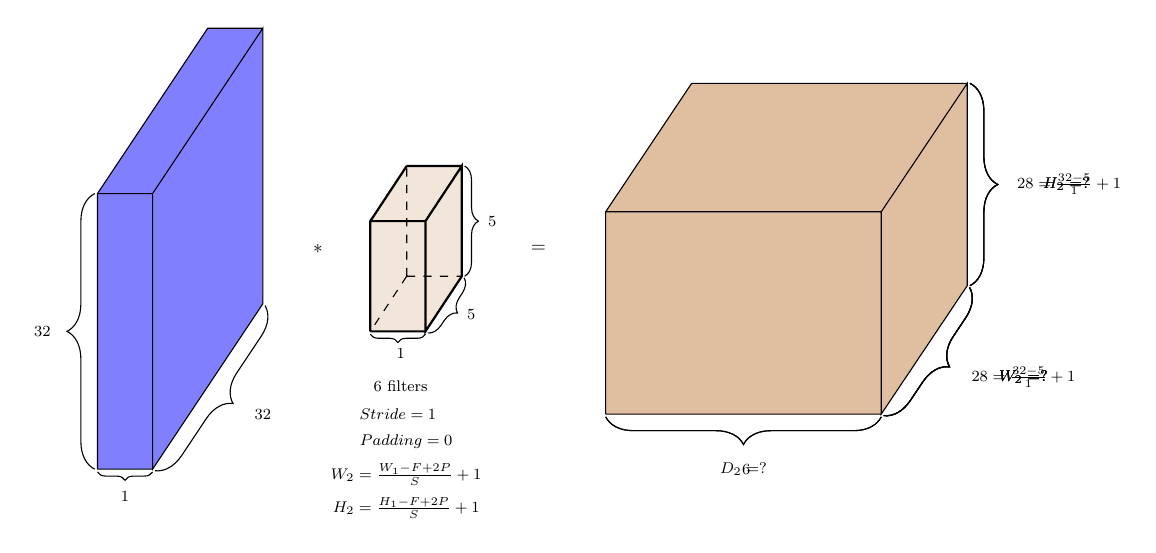
\begin{tikzpicture}[scale=0.7, transform shape]
\def\h{5}
\def\w{2}
\def\d{3}
\coordinate (A) at (0,0);
\coordinate (B) at (0,\h);
\coordinate (C) at (\w,\h+\d);
\coordinate (D) at (\w,\d);


\coordinate (A1) at (0+1,0);
\coordinate (B1) at (0+1,\h);
\coordinate (C1) at (\w+1,\h+\d);
\coordinate (D1) at (\w+1,\d);

\fill [draw=none, fill=blue!50] (A) -- (B) -- (C) -- (C1) -- (D1) -- (A1) -- cycle;
\draw (A) -- (B) -- (C) (A) -- (A1) (B) -- (B1) (C) -- (C1) (A1) -- (B1) -- (C1) -- (D1) -- cycle;

\draw [decorate,decoration={brace,amplitude=10pt,raise=1pt},xshift=0pt,yshift=0pt] (A) -- (B) node [black,midway,xshift=-1cm] {\footnotesize $32$};

\draw [decorate,decoration={brace,amplitude=3pt,raise=1pt},xshift=-4pt,yshift=0pt] (A1) -- (A) node [black,midway,yshift=-0.5cm] {\footnotesize $1$};

\draw [decorate,decoration={brace,amplitude=10pt,mirror,raise=1pt},xshift=0pt,yshift=0pt] (A1) -- (D1) node [black,midway,xshift=1cm,yshift=-0.5cm] {\footnotesize $32$};

\def\ha{2}
\def\wa{0.66}
\def\sa{1}
\def\wb{0.33}%shift
\def\sb{0.5}%shift
\def\hc{0.66}%next layer box
\def\wc{0.22}%next layer box size
\def\sc{0.33}
\def\xm{9} %distance of next box
\def\xmv{0.22}
\def\ymv{1}
\def\wid{1}


%layer1 feature map coordinates
\coordinate (A6) at (0+\xm+\xmv,0+\ymv);
\coordinate (B6) at (0+\xm+\xmv,\h-\sc);
\coordinate (C6) at (\w+\xm-\xmv,\h+\d-\ymv);
\coordinate (D6) at (\w+\xm-\xmv,\d+\sc);

\coordinate (A7) at (0+5+\xm+\xmv,0+\ymv);
\coordinate (B7) at (0+5+\xm+\xmv,\h-\sc);
\coordinate (C7) at (\w+5+\xm-\xmv,\h+\d-\ymv);
\coordinate (D7) at (\w+5+\xm-\xmv,\d+\sc);

\fill [draw=none, fill=brown!50] (A6) -- (B6) -- (C6) --  (D6) -- cycle;	


\def\xz{15}
\def\yz{-5}
		\coordinate (A2) at (0+\xz*\wb,0+\yz+\xz*\sb);
		\coordinate (B2) at (0+\xz*\wb,\ha+\yz+\xz*\sb);
		\coordinate (C2) at (\wa+\xz*\wb,\ha+\sa+\yz+\xz*\sb);
		\coordinate (D2) at (\wa+\xz*\wb,\sa+\yz+\xz*\sb);
		
		\coordinate (A3) at (0+1+\xz*\wb,0+\yz+\xz*\sb);
		\coordinate (B3) at (0+1+\xz*\wb,\ha+\yz+\xz*\sb);
		\coordinate (C3) at (\wa+1+\xz*\wb,\ha+\sa+\yz+\xz*\sb);
		\coordinate (D3) at (\wa+1+\xz*\wb,\sa+\yz+\xz*\sb);
		
		
		\fill [draw=none, fill=brown!50, fill opacity=0.4] (A2) -- (B2) -- (C2) -- (C3) -- (D3) -- (A3) -- cycle; 
			
		\draw[thick] (A2) -- (B2) -- (C2) (A2) -- (A3) (B2) -- (B3) (C2) -- (C3) (A3) -- (B3) -- (C3) -- (D3) -- cycle;
		\draw[dashed] (D2) -- (A2) (D2) -- (C2) (D2) -- (D3);

\draw [decorate,decoration={brace,amplitude=5pt,raise=1pt},xshift=0pt,yshift=0pt] (C3) -- (D3) node [midway,xshift=0.5cm] { \footnotesize{ $5$}};

\draw [decorate,decoration={brace,amplitude=3pt,raise=1pt},xshift=-4pt,yshift=0pt] (A3) -- (A2) node [black,midway,yshift=-0.4cm] { \footnotesize{ $1$}};

\draw [decorate,decoration={brace,amplitude=5pt,mirror,raise=1pt},xshift=0pt,yshift=0pt] (A3) -- (D3) node [black,midway,xshift=0.5cm,yshift=-0.2cm] { \footnotesize{$5$}};
		
		\node[] (input1) at (0+0.5+\xz*\wb,0+\yz+\xz*\sb-1) {\footnotesize{ $6$ filters}};
		\node[] (input1) at (0+0.5+\xz*\wb,0+\yz+\xz*\sb-1.5) {\footnotesize{$Stride = 1$}};
		\node[] (input1) at (0+0.65+\xz*\wb,0+\yz+\xz*\sb-2) {\footnotesize{$Padding = 0$}};	
		\node (m1) at (0+0.65+\xz*\wb,0+\yz+\xz*\sb-2.6) {\footnotesize $W_2 = \frac{W_1-F+2P}{S}+1$};
		\node (m1) at (0+0.65+\xz*\wb,0+\yz+\xz*\sb-3.2) {\footnotesize $H_2 = \frac{H_1-F+2P}{S}+1$};
		%\node (m1) at (0+0.65+\xz*\wb,0+\yz+\xz*\sb-3.8) {\footnotesize $D_2 = K$};

\node (m1) at (4,4) {$*$};

\node (m1) at (8,4) {$=$};

		\fill [draw=none, fill=brown!50] (A6) -- (B6) -- (C6) -- (C7) -- (D7) -- (A7) -- cycle;
		\draw [black] (A6) -- (B6) -- (C6) (A6) -- (A7) (B6) -- (B7) (C6) -- (C7) (A7) -- (B7) -- (C7) -- (D7) -- cycle;

\onslide<1>{

\draw [decorate,decoration={brace,amplitude=10pt,raise=1pt},xshift=0pt,yshift=0pt] (C7) -- (D7) node [midway,xshift=1.8cm] { \footnotesize{$H_2 = ?$}};

\draw [decorate,decoration={brace,amplitude=10pt,raise=1pt},xshift=-4pt,yshift=0pt] (A7) -- (A6) node [black,midway,yshift=-1cm] { \footnotesize{$D_2 = ?$}};

\draw [decorate,decoration={brace,amplitude=10pt,mirror,raise=1pt},xshift=0pt,yshift=0pt] (A7) -- (D7) node [black,midway,xshift=1.8cm,yshift=-0.5cm] { \footnotesize{$W_2 = ?$}};

}

\onslide<3->{

\draw [decorate,decoration={brace,amplitude=10pt,raise=1pt},xshift=0pt,yshift=0pt] (C7) -- (D7) node [midway,xshift=1.8cm] { \footnotesize{ $28 = \frac{32-5}{1}+1$}};
\onslide<3>{


\draw [decorate,decoration={brace,amplitude=10pt,mirror,raise=1pt},xshift=0pt,yshift=0pt] (A7) -- (D7) node [black,midway,xshift=1.8cm,yshift=-0.5cm] { \footnotesize{$W_2 = ?$}};
}
}
\onslide<2->{
\draw [decorate,decoration={brace,amplitude=10pt,raise=1pt},xshift=-4pt,yshift=0pt] (A7) -- (A6) node [black,midway,yshift=-1cm] { \footnotesize{ $6$}};
\onslide<2>{
\draw [decorate,decoration={brace,amplitude=10pt,raise=1pt},xshift=0pt,yshift=0pt] (C7) -- (D7) node [midway,xshift=1.8cm] { \footnotesize{$H_2 = ?$}};

\draw [decorate,decoration={brace,amplitude=10pt,mirror,raise=1pt},xshift=0pt,yshift=0pt] (A7) -- (D7) node [black,midway,xshift=1.8cm,yshift=-0.5cm] { \footnotesize{$W_2 = ?$}};
}}
\onslide<4->{
\draw [decorate,decoration={brace,amplitude=10pt,mirror,raise=1pt},xshift=0pt,yshift=0pt] (A7) -- (D7) node [black,midway,xshift=1.8cm,yshift=-0.5cm] { \footnotesize{$28 = \frac{32-5}{1}+1$}};
}
%\node (m1) at (2.5,-1) {$W_2 = \frac{W_1-F+2P}{S}+1$};

\end{tikzpicture}
\end{center}
		\end{overlayarea}
		
	\end{columns}
\end{frame}
